% Définition du document
\documentclass{article}

% Paquets nécessaires
\usepackage{amsmath} % Pour les mathématiques
\usepackage{amsfonts} % Pour les polices mathématiques supplémentaires
\usepackage{amssymb} % Pour les symboles mathématiques
\usepackage{tikz} % Pour les graphiques vectoriels
\usepackage{pgfplots} % Pour les graphiques en 2D et 3D
\usepackage{setspace} % Pour l'espacement des lignes
\usepackage{color} % Pour les couleurs de texte
\usepackage{mathrsfs} % Pour les lettres cursives en mathématiques
\usepackage{blindtext}
\usetikzlibrary{automata, positioning, arrows}
% Configuration des bibliothèques TikZ
\usetikzlibrary{positioning,quotes}
\usepgfplotslibrary{fillbetween}
\pgfplotsset{compat=1.18}

% Configuration de la page
\usepackage[letterpaper,total={6in, 8in}]{geometry}

% Informations sur le document
\title{Devoir 2}
\author{Emeric Laberge, Arpad Botond Rigo}
\date{\today}

% Début du document
\begin{document}

% Page de titre
\begin{titlepage}
\begin{center}
\vspace*{1cm}

\Huge
\textbf{Devoir 3}

\vspace{0.5cm}
\LARGE

\vspace{1.5cm}

\textbf{Emeric Laberge}

\vfill

Dans le cadre du cours\\
IFT 1575 


\vspace{0.8cm}


\includegraphics[width=0.4\textwidth]{Université-de-Montréal.jpg}

\Large
Département d'informatique et de recherche opérationnelle\\
Université de Montréal\\
Canada\\
24 mars 2023 

\end{center}
\end{titlepage}


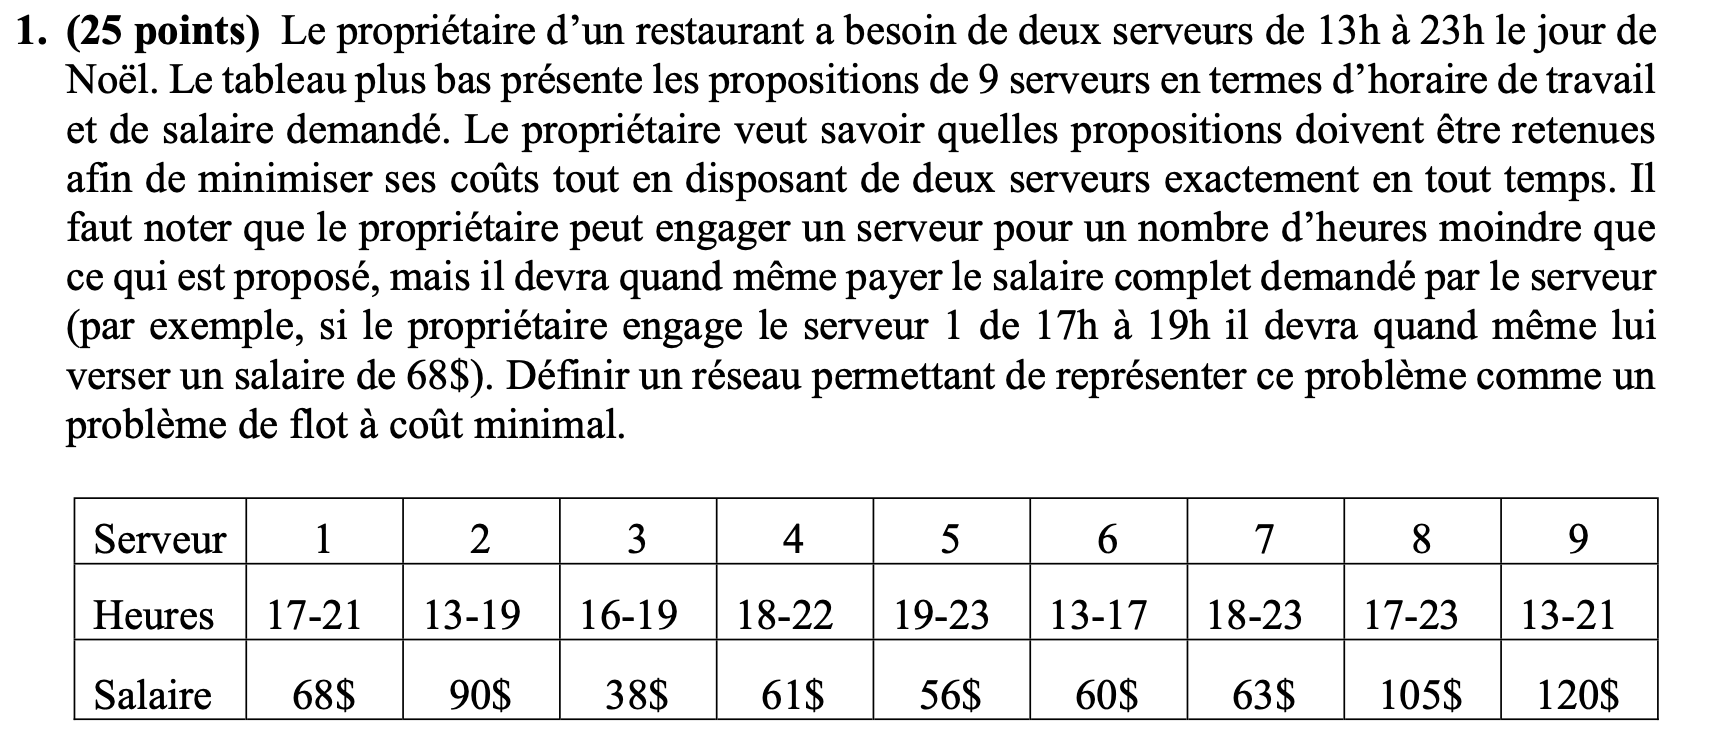
\includegraphics[width=1 \textwidth]{num1} 
\pagebreak


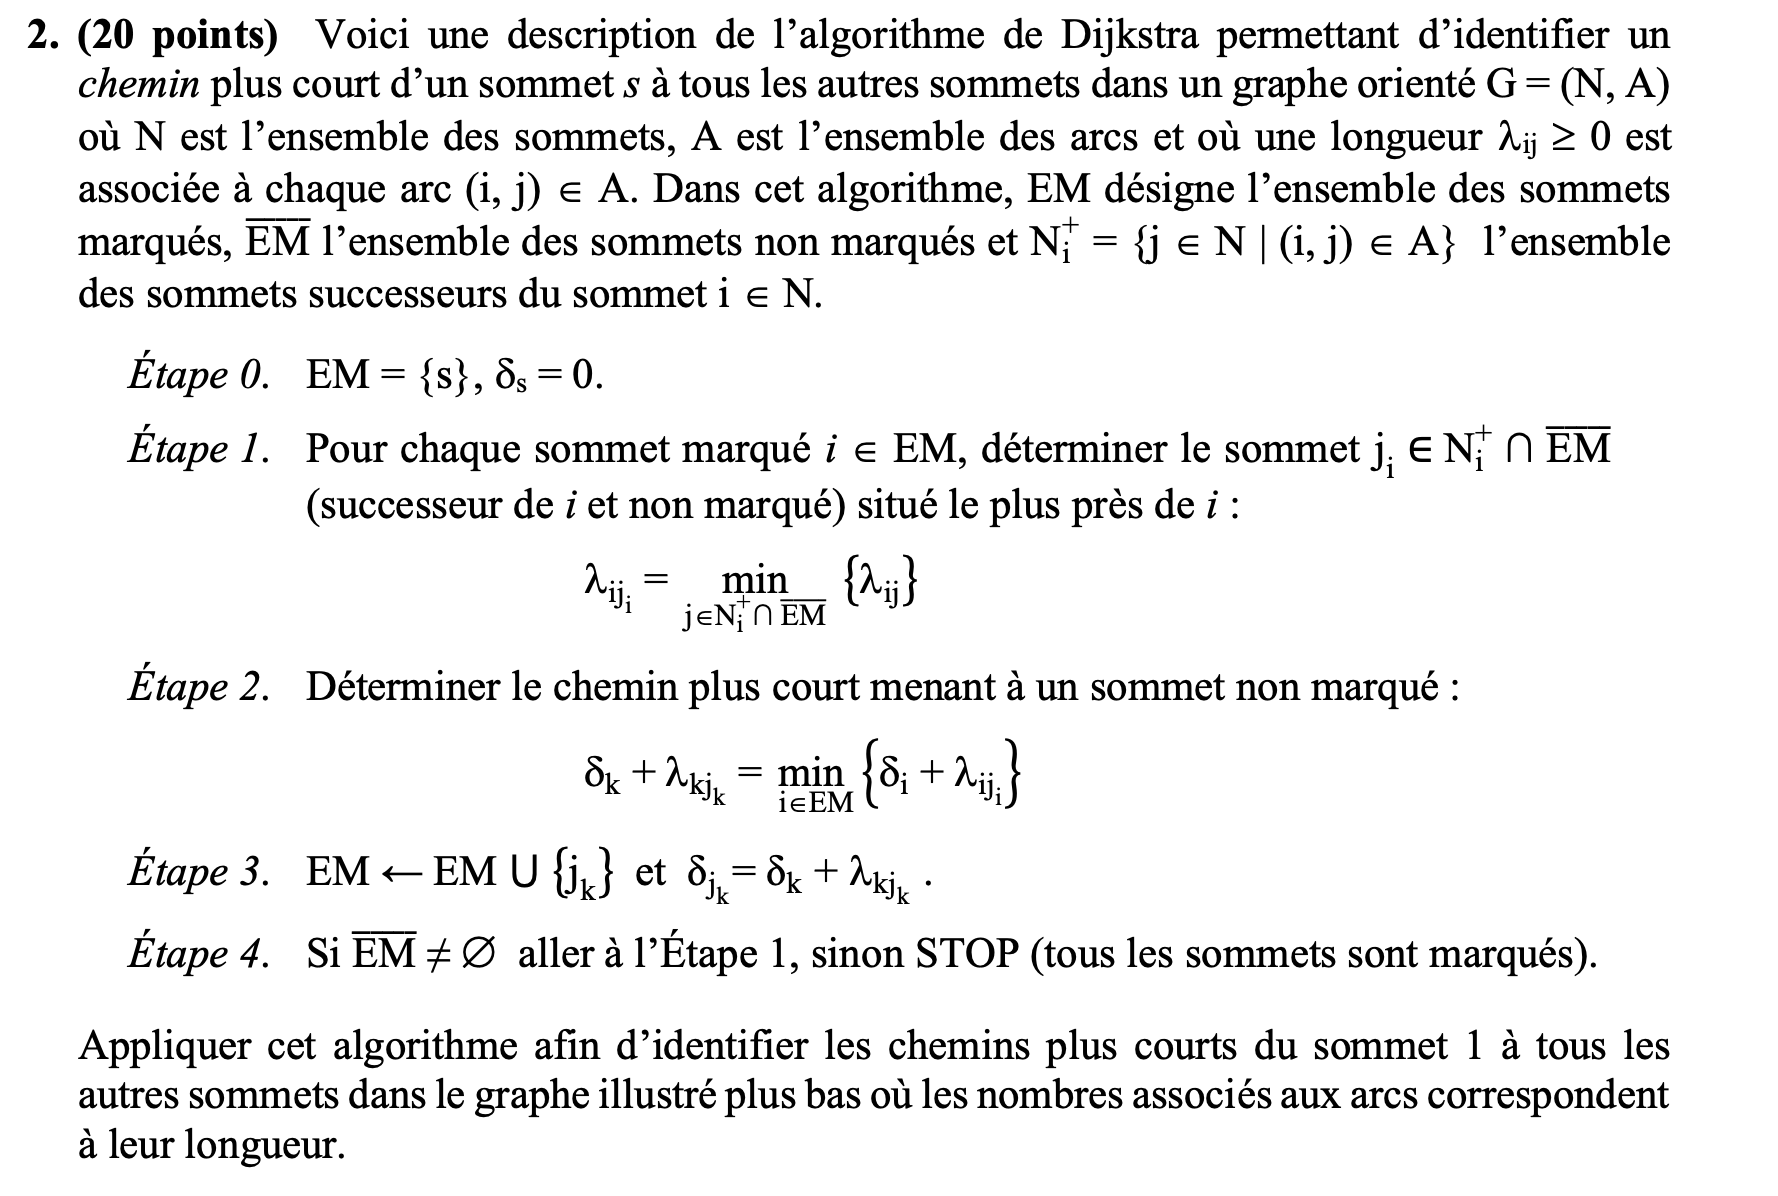
\includegraphics[width=1 \textwidth]{num2} 
\pagebreak

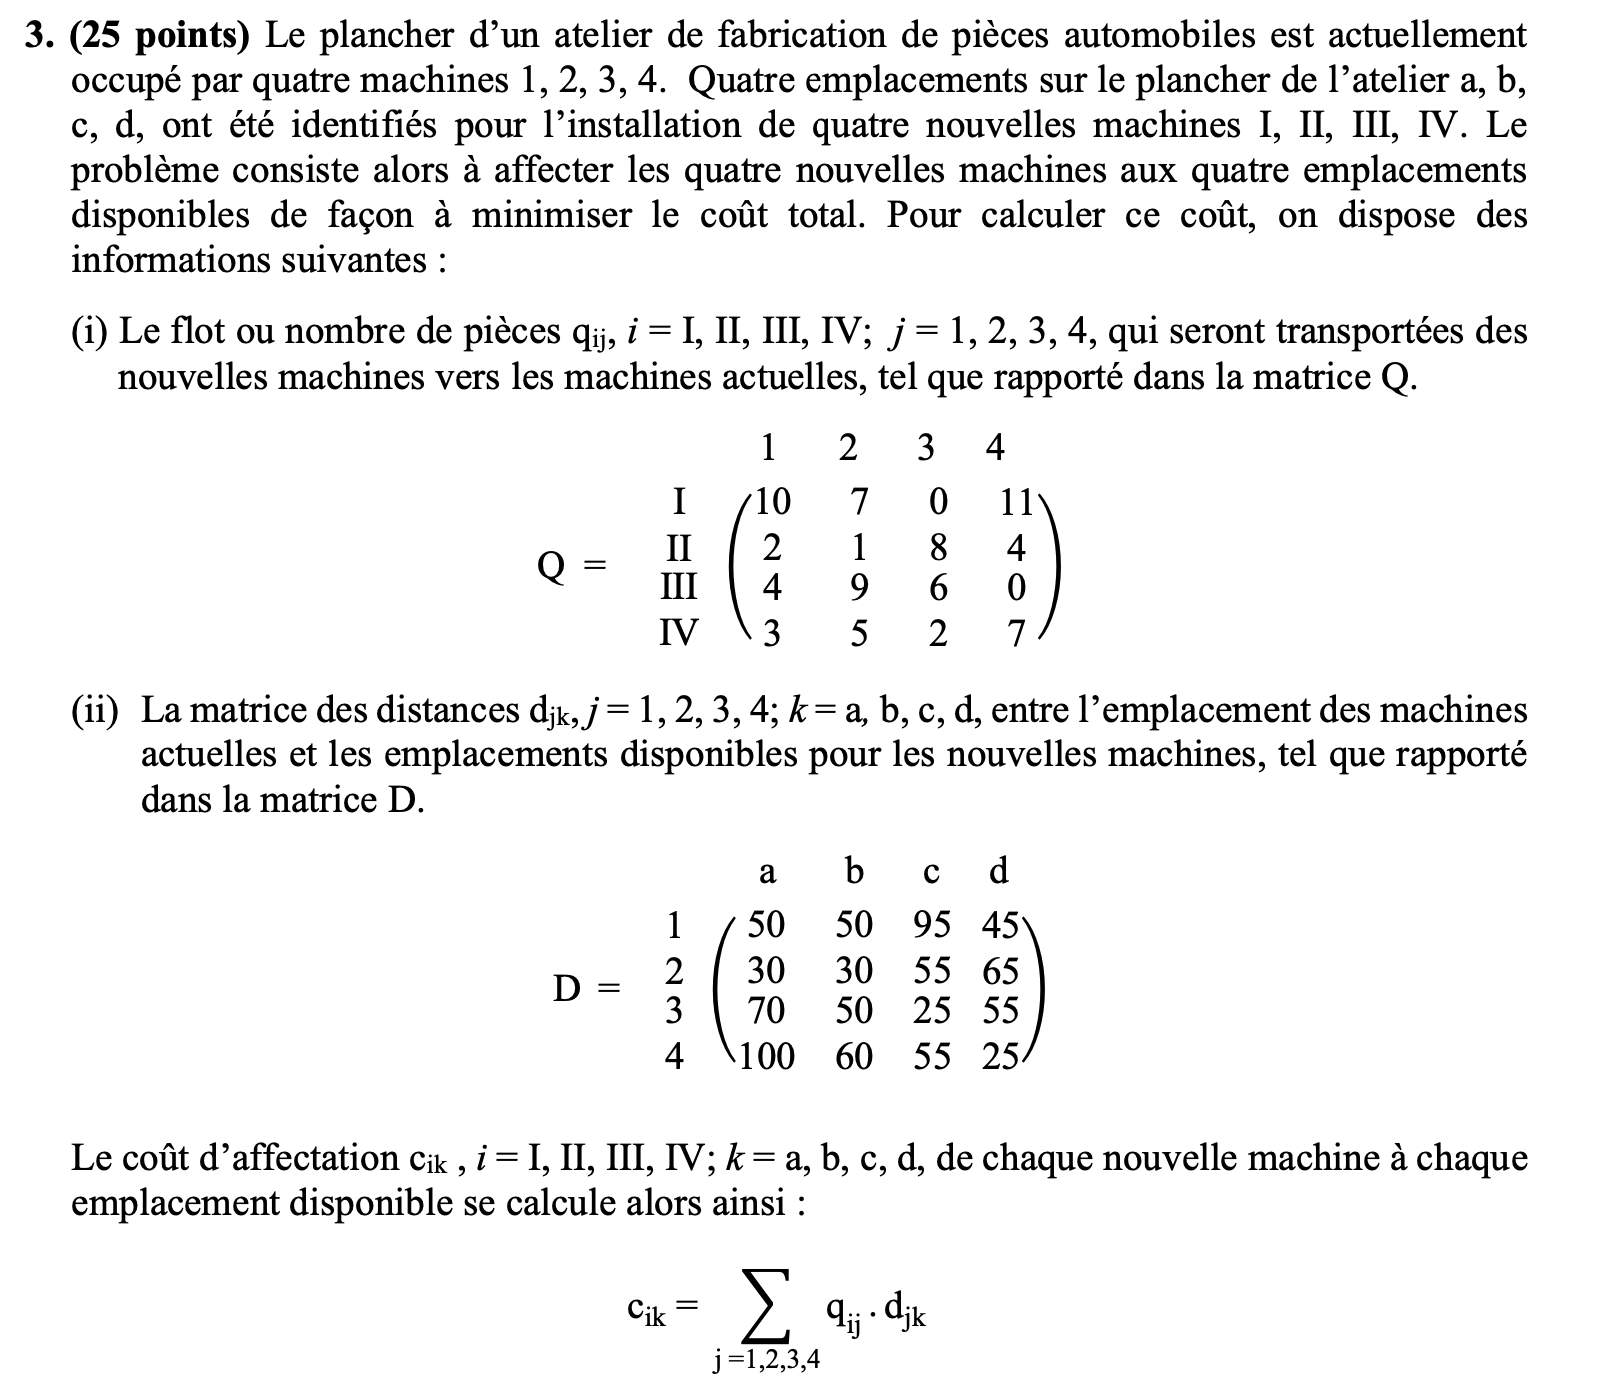
\includegraphics[width=1 \textwidth]{num3}
\subsection*{(a)} 
\pagebreak

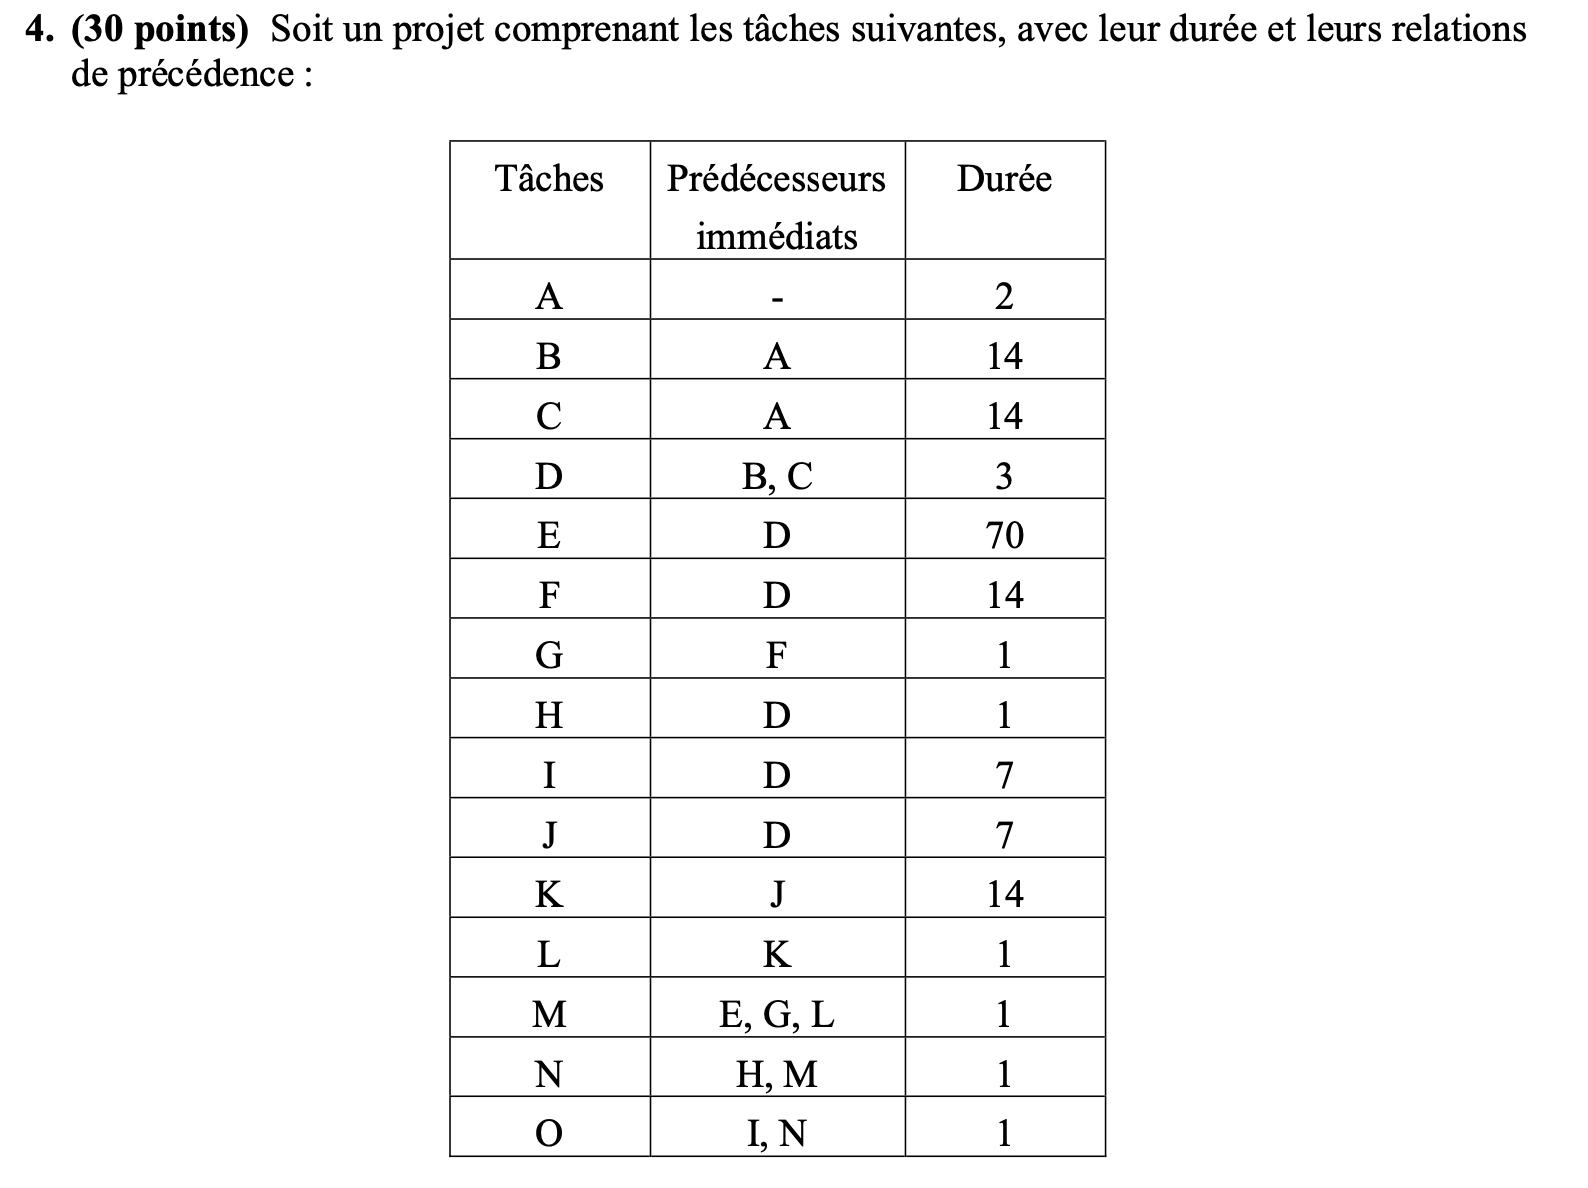
\includegraphics[width=1 \textwidth]{num4} 
\end{document}